\documentclass[12pt]{article}

\usepackage[utf8]{inputenc}
\usepackage{amsmath,amssymb}
\usepackage[margin=1in]{geometry}
\usepackage{lmodern}
\usepackage{microtype}
\usepackage{fancyhdr}
\usepackage{titlesec}
\usepackage{hyperref}
\usepackage{graphicx}

\title{Communication Systems Exam}
\author{}
\date{\today}

\begin{document}
	
	\maketitle
	
	\section{Question 1}
	
	Create a conceptual diagram of a communication system, including transmitter, receiver, and channel, and the intermediate stages necessary to conceptually place the following fundamental relationships:
	
	\begin{enumerate}
		\item $\overline{L} \geq H(\mathcal{S})$
		\item $C = B\log_2\left(1+ \frac{S}{N}\right)$
		\item $H = \sum_{k = 0}^{K - 1} p_k \log_2\left(\frac{1}{p_k}\right)$
	\end{enumerate}
	
	Briefly define the meaning of each relationship, explaining the units of measurement for each involved magnitude.
	
	\vspace{10cm}
	
	\section{Question 2}
	
	Describe, using a sequence diagram, the process of establishing a TCP connection and the process of closing a connection between a client and a server. Show both sequences of messages on the following TCP state machine:
	
	\begin{figure}[ht]
		\centering
		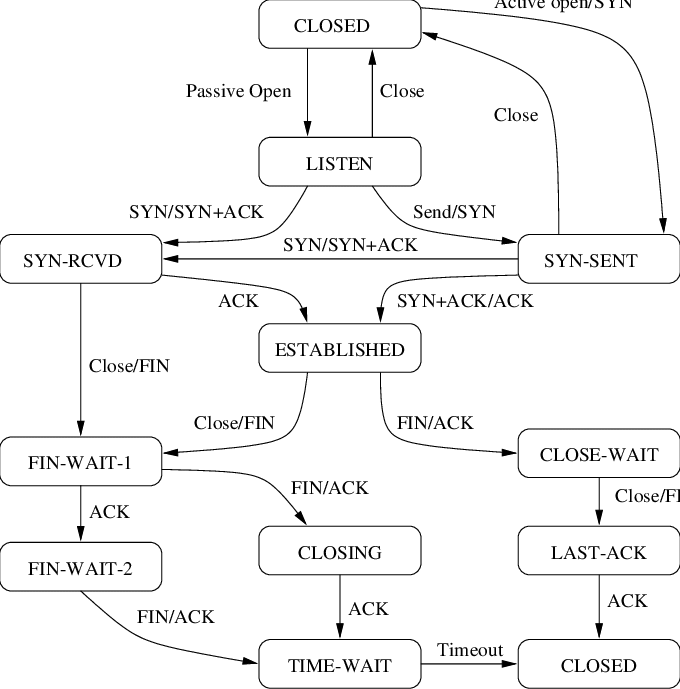
\includegraphics[scale=0.5]{tcp.jpg}
		\caption{TCP state machine.}
		\label{fig:tcp}
	\end{figure}
	
	\section{Question 3}
	
	Create two diagrams that highlight the difference between the Symmetric Key Cryptography system and the Public Key Cryptography system for communication between two different users, A and B, who need to send confidential information to a third user, C, over an insecure network. Describe one advantage and one disadvantage of each method.
	
\end{document}
